\documentclass[a4paper, 12pt]{article}
\usepackage[utf8]{inputenc}
\usepackage[T1]{fontenc}
\usepackage{textcomp, color, amsmath, amssymb, tikz, subfig, float, mathrsfs}
\usepackage{xcolor}
\usepackage{amsfonts}
\usepackage{graphicx}
\usepackage{listings}
\usepackage{ragged2e}
\usepackage{amsmath}
\usepackage[export]{adjustbox}
\usepackage[]{esint}
\usepackage{hyperref}
\usepackage[skins,theorems]{tcolorbox}
\usepackage{cite}
\usepackage{algorithm}
\usepackage{algorithmicx}
\usepackage{algpseudocode}
\usepackage{subfig}% http://ctan.org/pkg/subfig
\newsubfloat{figure}
%Tikzcommands
\usepackage{tikz}
\usetikzlibrary{shapes.geometric, arrows}
\tikzstyle{startstop} = [rectangle, rounded corners, minimum width=3cm, minimum height=1cm,text centered, draw=black, fill=red!30]
\tikzstyle{io} = [trapezium, trapezium left angle=70, trapezium right angle=110, minimum width=3cm, minimum height=1cm, text centered, draw=black, fill=blue!30]
\tikzstyle{process} = [rectangle, minimum width=3cm, minimum height=1cm, text centered, draw=black, fill=orange!30]
\tikzstyle{decision} = [diamond, minimum width=3cm, minimum height=1cm, text centered, draw=black, fill=green!30]
\tikzstyle{arrow} = [thick,->,>=stealth]




\tcbset{highlight math style={enhanced,
  colframe=red,colback=white,arc=10pt,boxrule=0.5pt, hbox}}

\definecolor{lightgray}{gray}{0.75}

\newcommand\greybox[1]{%
  \vskip\baselineskip%
  \par\noindent\colorbox{lightgray}{%
    \begin{minipage}{\textwidth}#1\end{minipage}%
  }%
  \vskip\baselineskip%
}
	
\newcommand{\vertfig}[2][]{%
  \begin{minipage}{5in}\subfloat[#1]{#2}\end{minipage}}
  
\newcommand{\horizfig}[2][]{%
  \begin{minipage}{3in}\subfloat[#1]{#2}\end{minipage}}


\begin{document}



\author{Kristian Tuv}
\title{Investigating the properties of an argon liquid using molecular dynamics}
\maketitle
Link to the code: \url{https://github.com/kristtuv/FYS3150}
\newpage
\tableofcontents
\newpage
\section{Abstract}
We have used the molecular dynamics model with the Lennard-Jones potential and periodic boundary conditions to find properties of an argon-liquid. The liquid is initalized as a FCC-crystal consisting of 1372 atoms. Every atom was given a speed using the Boltzmann speed distribution and the total momentum of the system was set to zero by subtracting the mean speed of the atoms from every atom. The velocity verlet algorithm was used to calculate the velocities and positions at every timestep.\\

We found the density in the liquid to be 1823.25 $kg/m^3$, the energy to be conserved and by looking at the temperature ratio of the final temperatures and the intial temperatures combined with the value of the diffusion constant we found the phase transition of the liquid to happen close to 300 K. The measurements are however highly uncertain because of the relatively small amount of data gathered in the simulation.

\section{Introduction}


In this project we will implement a model called molecular dynamics (MD). MD  allows us to study the dynamics of atoms and explore the phase space. The atoms and molecules are allowed to interact for a fixed	period of time, giving a view of the dynamical evolution of the system. Analytically we are only able to calculate the interactions between a couple of atoms, but with a sufficiently powerful computer we are able to calculate the interactions between millons of atoms. With the computing power we have available in this project however, we are only able to calculate the interactions of up to a few thousand atoms, but by applying periodic boundary conditions we can view the system as infinit size.\\

The method of molecular dynamics was developed within the field of theoretical physics in the late 1950s\cite{MD} but is applied today mostly in chemical physics, material science and the modelling of biomolecules. For instance MD can be used in the modelling of gas hydrates in ice or the interaction of molecules in the human body.\\

In this project we will build a model of an argon-liquid finding different properties of the liquid at different temperatures, most importantly we will try to find the temperature at which the liquid experiences a phase transition.

\newpage
\section{ Theory And Methods}
\subsection{Molecular Dynamics Units}
In our simulations we use molecular dynamics units. In molecular dynamics units our goal is to make Boltzmann's constant $k_B = 1 J/K$. \\The reason we use this units are that we are working with extremely small values on the atomic scale and this would not be nummerically stable.\\
\\ \\
\begin{tabular}{| c | c |}
\hline
\textbf{MD-units}  & \textbf{SI-units}\\
\hline
1 temperature unit & 119.735 K\\
\hline
1 mass unit & 1.66054 $\times 10^{-27}$ kg\\
\hline
1 length unit(1 Angstrom) & $10^{-10}\textit{m} $\\ \hline
1 time unit & 1.00224 $\times 10^{-13}$ s \\ \hline
1 speed unit & 997.765 m/s\\ \hline
1 force unit & 1.653 $\times 10^{-11} N$\\ \hline
1 pressure unit & 1.653 $\times 10^{9} N/\textit{m}^2$\\ \hline
1 energy unit & 6 1.651 $\times 10^{-21}$ J\\
\hline
\end{tabular}
\\


\subsection{Mathematical Theory}

\subsubsection{Argon Crystal Structure}
When setting up our system, we use face centered cubic unit cells to initialize the atoms in a argon crystal. Each unit cell of size $b = 5.26$ Angstrom consists of four atoms initalized with the local coordinates\\
\begin{align}
\vec{r}_{1} &= 0\hat{i} + 0\hat{j} + 0\hat{k} \\
\vec{r}_{2} &= \frac{b}{2}\hat{i} + \frac{b}{2}\hat{j} + 0\hat{k} \\
\vec{r}_{3} &= 0\hat{i} + \frac{b}{2}\hat{j} + \frac{b}{2}\hat{k} \\
\vec{r}_{4} &= \frac{b}{2}\hat{i} + 0\hat{j} + \frac{b}{2}\hat{k}
\end{align}
We can now create $N_x \times N_y \times N_z$ such unit cells next to each other to form a larger crystal so that the origin of unit cell $(i,j,k)$ is

\begin{align}
	\mathbf{R}_{i,j,k} = i \hat{\mathbf{u}}_1 + j \hat{\mathbf{u}}_2 + k \hat{\mathbf{u}}_3,
\end{align}
where $i=0,1,..., N_x-1, j=0,1,..., N_y-1, k=0,1,..., N_z-1$. The unit vectors of the unit cells are scaled with the lattice constant $b$ so that

\begin{align}
	\hat{\mathbf{u}}_1 = b\hat{\mathbf{i}}, \quad \hat{\mathbf{u}}_2 = b\hat{\mathbf{j}}, \quad \hat{\mathbf{u}}_3 = b\hat{\mathbf{k}}.
\end{align}
 The number of atoms in the structure becomes $4\times N_x \times N_y \times N_z$.\\
In our simpulations we will keep the number of atoms N, the volume V and the energy E constant. That is, we are looking at the microcanonical ensemble. We want to work with the microcanonical ensemble to have full control over our system at all times. \\
Even though the system is initialized with a crystalline structure, we are using a potential that allows the atoms to move far more than they would in a solid so we are looking at a liquid. This means when looking for a phase transition at higher temperatures, we are looking for the boiling point of Argon.\\
In tables on the internet \cite{ArgonBoiling} we find that the boiling point of Argon is 87 K, however, as we will see in section 3.2.4, our system has a very high pressure which makes the boiling point shift to a higher temperature.

\begin{figure}
\centering
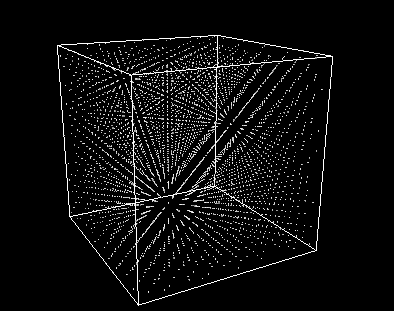
\includegraphics[width = 0.6\textwidth]{/Users/Tuv/Documents/Programming/FYS3150/Project5/argonstructure}
\caption{FCC-crystal of argon containing 4000 atoms. In our simulations we will be using 1372 atoms}
\end{figure}
\subsubsection{Equipartition Theorem}
The Equipartition theorem\cite{Equipartition} states that\\
If a system contains N molecules, each with f degrees of freedom, and there are no other (non-quadratic) temperature-dependent forms of energy, then its total thermal energy is
\begin{equation}
U_{thermal} = N_{atoms} \cdot f \cdot \frac{1}{2} kT
\end{equation}
We only consider the translational degrees of freedom, which makes f = 3 and the energy U is the kinetic energy $E_k$. We solve for T and get an expression we can use to find the temperature of the system
\begin{equation}
T = \frac{2}{3}\frac{E_k}{kN_{atoms}}
\end{equation}
\subsubsection{The Boltzmann Speed Distribution}
The ergodic hypothesis states that the simulation will have an equiprobable chance of entering all possible microstates over a longer period of time when we are looking at an idel gas (a noninteracting gas). This means that we can use the Boltzmann speed distribution, 

$$P(v_i ) = \left (\frac{m}{2\pi k_b T}\right )^{1/2} e^{\left ( \frac{-mv_i^2}{2k_B T}\right )}$$

which we recognize as the a normal distribution with zero mean and standard diviation $\sigma = \sqrt{k_B T/m}$,  to initialize the speed of each atom.\\
 $P(v_i )$ is the probability of an atom having the speed $v_i$ in the i-direction. m is the mass of the atom, $k_B$ is the Boltzmann constant and T is the temperature.
\subsubsection{System Density and Van der Waals Equation for Liquid-Gas Systems}

The density $\rho$ is given by the number of atoms $4\times N_x \times N_y \times N_z = 4N_{UnitCells}^3$ times their individual masses m devided by the size of the system. Beacuse all the individual masses are equal we get
\begin{equation}
\rho = \frac{M}{V} = \frac{4mN_{UnitCells}^{3}}{(bN_{UnitCells})^{3}} = \frac{4m}{b^{3}}
\end{equation}
We can see this equation only depends on the lattice constant b and the mass of the atoms. If we use the mass of an argon atom $m = 39,948 u = 6.6335209 \times 10^{-26} kg$ and the lattice constant $b = 5.26 A = 5.26 \times 10^{-10} m$, whe get the density of our system: $$\rho = 1823.25 \mathit{kg/m^3}$$

To calculate the pressure we use the van der Waals Model, which is the most famous model for liquid-gas systems. This is simply a modification of the ideal gas law which takes molecular interactions into account in an approximate way.
\begin{equation}
P = \frac{N k_B T}{V - N\gamma} - \frac{aN^{2}}{V^{2}}
\end{equation}
Because a fluid can not be compressed all the way down to zero volume, the volume is limited to a minimum value of N$\gamma$, where N is the number of atoms and $\gamma$ is a constant which depends on the type of atoms we are looking at.\\
$ \frac{aN^{2}}{V^{2}}$ account for the short-range attractive forces between atoms when they are not touching.\\

In our system $V = (N_{UnitCells}b)^3$ and $N = 4N_{UnitCells}^3$\\
We substitue this into our pressure-equation and get:
\begin{equation}
P = \frac{4k_B T}{b^{3} - 4\gamma} - \frac{16a}{b^{6}}
\end{equation}
From tables on the internet\cite{Argon} we find that $\gamma$ = 0.03201 L/mol and $a = 1.355 L^2 bar/mol^2$.\\
By changing the units of the constants to $\gamma = [m^3]$ and $a = [m^6 Pa] $, we can plot this equation for different T-values for our system which can be seen in figure 2\\

\begin{figure}[H]
\centering
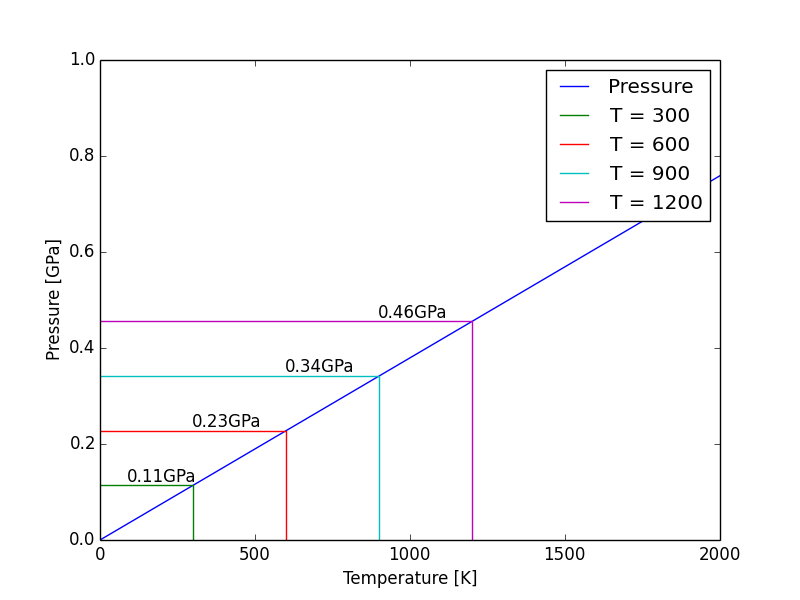
\includegraphics[width=0.7\textwidth]{/Users/Tuv/Documents/Programming/FYS3150/Project5/molecular-dynamics-fys3150-master/PressureVanderWaals.png}
\caption{The van der Waals equation for different temperatures. Some temperatures and corresponding pressures have been marked in the plot. We see that for our system, room temperature(300 K) already corresponds to an extremely high pressure}
\end{figure}
 
\subsubsection{The Leonnard-Jones Potential}
The Lennard-Jones potential\cite{LennardJones} is commenly used in molecular dynamics calculations. This is beacause we want a potential that is weakly interacting at large distances and strongly repulsive at short distances.
\begin{equation}
U(r_{ij}) = 4\epsilon \left [\left (\frac{\sigma}{r_{ij}} \right )^{12} - \left ( \frac{\sigma}{r_{ij}} \right )^{6}\right ]
\end{equation}
$r_{ij} = |\mathbf{r}_i - \mathbf{r}_j |$ is the distance between two atoms, $\epsilon$ is the depth of the potential well, $\sigma$ is the distance at which the potential is zero.\\
\\
The force is calculated by taking the negative gradient of the potential:
\begin{equation}
\mathbf{F}_{ij} = - \nabla U(r_{ij} ) = 24\epsilon\frac{1}{r_{ij}^{2}} \left [ \left ( 2\frac{\sigma}{r_{ij}}\right )^{12} - \left (  \frac{\sigma}{r_{ij}} \right )^{6} \right ]\mathbf{r}_{ij}
\end{equation}

\begin{figure}[H]
\centering
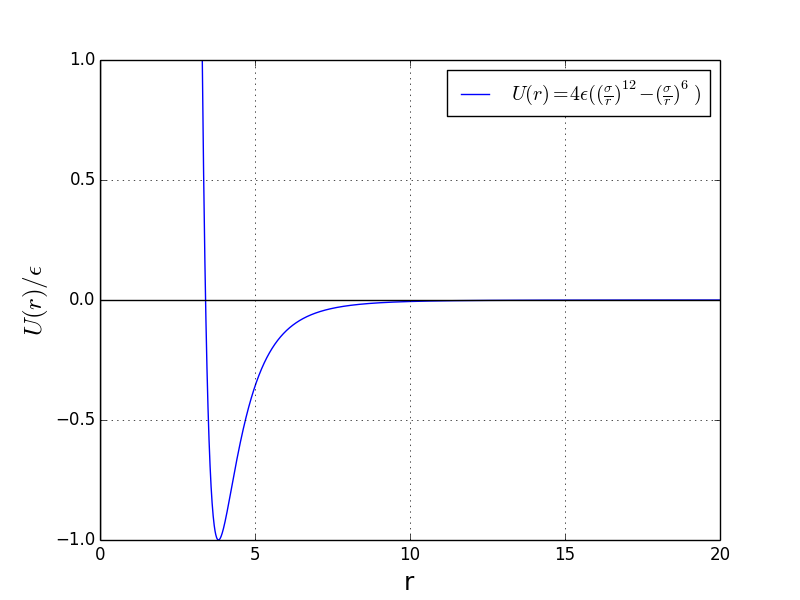
\includegraphics[width=0.8\textwidth]{/Users/Tuv/Documents/Programming/FYS3150/Project5/molecular-dynamics-fys3150-master/Lennardjones.png}
\caption{The Lennard-Jones potential with $\epsilon = 1 [119.8 K]$ and $\sigma = 3.405 [A]$}
\end{figure}


\subsubsection{The Diffusion Constant}
The diffusion constant tells us the rate of mixing in a fluid or gas. We will be using the Einstein relation that relates the mean square displacement to the diffusion constant\cite{DiffusionConstant} 
\begin{equation}
\langle r^2 (t) \rangle = 2n_{dim} D t = 6Dt \rightarrow D = \frac{\langle r^2 (t) \rangle}{6t}
\end{equation}



Where D is the diffusion constant, t is time, $n_{dim}$ is the number of dimentions and
\begin{equation}
r_i^2 (t)  = |\mathbf{r}_i (t) - \mathbf{r}_i (t)|^2
\end{equation} is the mean square displacement for atom i.\\
We see from this equation that D tells us how much the atoms are moving away from their initial positions. For a liquid or a solid the value of D should be close to or equal to zero.
\subsection{Nummerical Calculations}
\subsubsection{ProgramFlow}
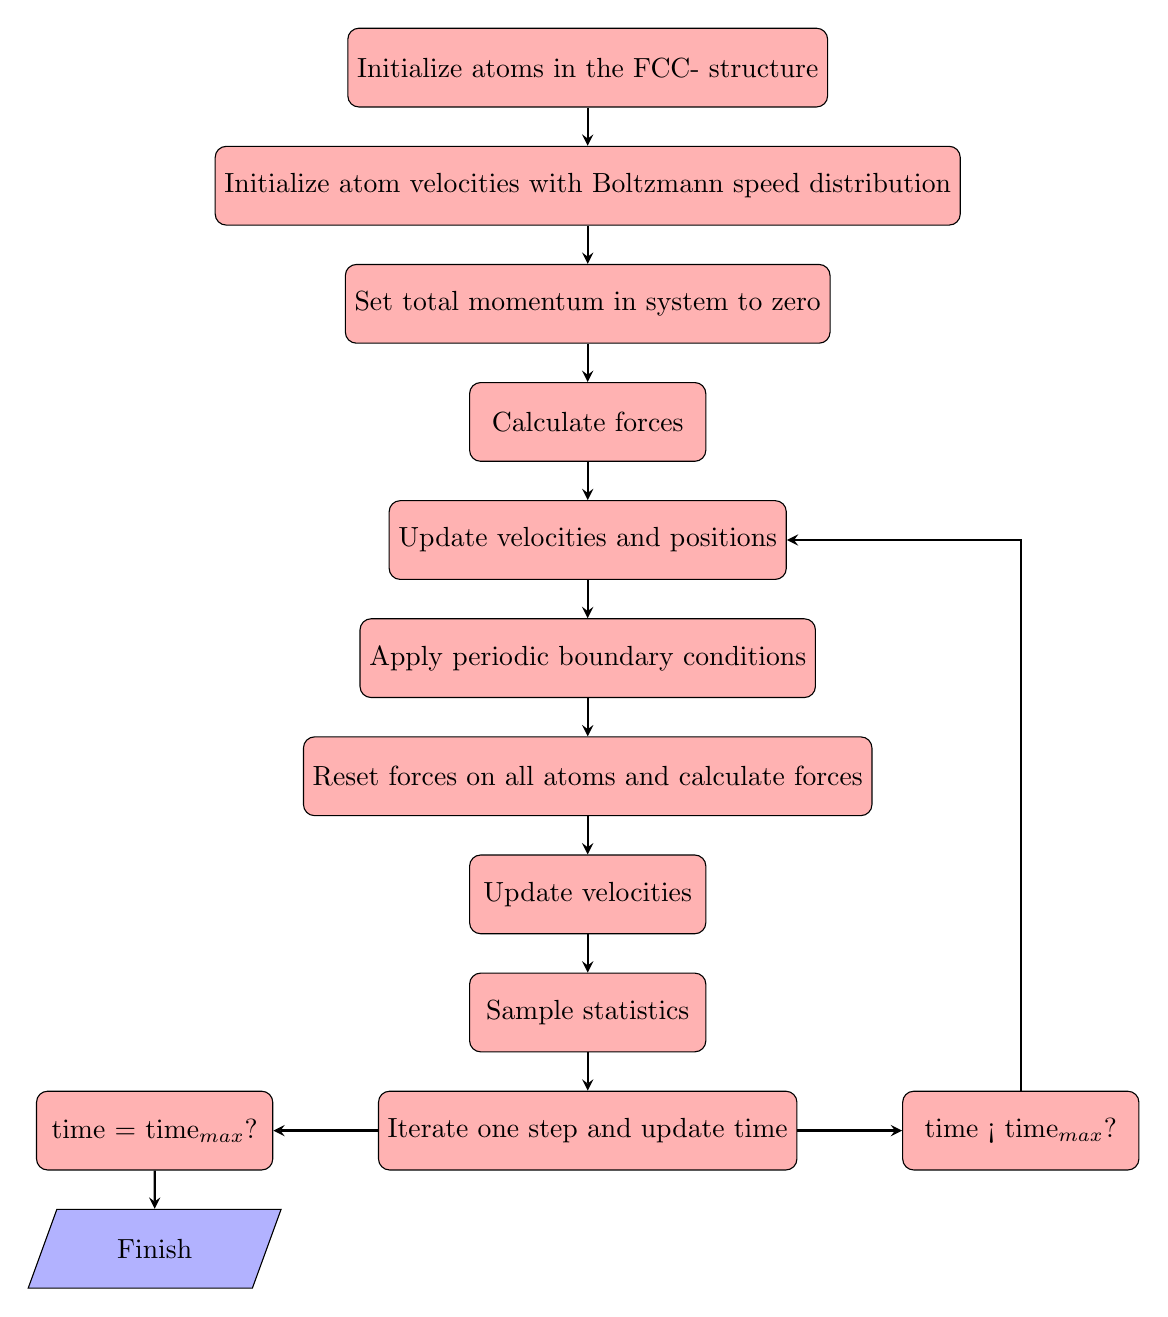
\begin{tikzpicture}[node distance=1.5 cm]
\node (step1) [startstop] {Initialize atoms in the FCC- structure};
\node (step2) [startstop, below of=step1] {Initialize atom velocities with Boltzmann speed distribution};
\node (step3) [startstop, below of=step2] {Set total momentum in system to zero};
\node (step4) [startstop, below of=step3] {Calculate forces};
\node (step5) [startstop, below of=step4] {Update velocities and positions};
\node (step6) [startstop, below of=step5] {Apply periodic boundary conditions};
\node (step7) [startstop, below of=step6] {Reset forces on all atoms and calculate forces};
\node (step8) [startstop, below of=step7] {Update velocities};
\node (step9) [startstop, below of= step8]{Sample statistics};
\node (step10) [startstop, below of=step9] {Iterate one step and update time};
\node (step11) [startstop, right of=step10, xshift=4cm] { time < time$_{max}$?};
\node (step12) [startstop, left of=step10, xshift= -4cm] {time = time$_{max}$?};
\node (step13) [io, below of=step12] {Finish};


\draw [arrow] (step1) -- (step2);
\draw [arrow] (step2) -- (step3);
\draw [arrow] (step3) -- (step4);
\draw [arrow] (step4) -- (step5);
\draw [arrow] (step5) -- (step6);
\draw [arrow] (step6) -- (step7);
\draw [arrow] (step7) -- (step8);
\draw [arrow] (step8) -- (step9);
\draw [arrow] (step9) -- (step10);
\draw [arrow] (step10) -- (step12);
\draw [arrow] (step10) -- (step11);
\draw [arrow] (step12) -- (step13);
\draw [arrow] (step11) |- (step5);
\end{tikzpicture}
\newpage
\subsubsection{The Velocity Verlet algortihm}
\begin{algorithm}[H]
\caption{Velocity Verlet algorithm}
\label{alg:verlet_algorithm}
\begin{algorithmic}[1]
\If{We are on the first run, $t_0$}
	\State We make sure we have an initial setup, and calculate forces $\mathbf{F}$  for the initial positions and velocities.
\EndIf
\For{atom in atomsarray}
\State $\mathbf{v}(t+\Delta t/2) = \mathbf{v}(t) + \frac{\mathbf{F}}{m}\frac{\Delta t}{2}$
\State $\mathbf{r}(t+\Delta t) = \mathbf{r}(t) + \mathbf{v}(t + \Delta t/2) \Delta t$
\EndFor
\State Update forces based on the new positions and velocities, $\mathbf{F}(t+\Delta t)$
\State Update boundary conditions
\For{atom in atomsarray}
\State $\mathbf{v}(t+\Delta t) = \mathbf{v}(t+\Delta/2) + \frac{\mathbf{F}(t+\Delta t)}{m}\frac{\Delta t}{2}$
\EndFor
\end{algorithmic}
\end{algorithm}

\subsubsection{Conservation Of Momentum}
The Boltzmann speed distribution does in general not produse a system of atoms with a conserved total momentum. In order to conserve the momentum i subtracted to mean momentum from all the particles.

\subsubsection{Real distances}
When using periodic boundary conditions we have to be careful when calculating the distances between the atoms, and the distance an atom has moved from the initial position. We want to simulate a system of "infinite" size, and when an atom moves through the boundary on the right side we imagine it countinuing into an equal system even though it reappears on the left side.
\begin{figure}[H]
\centering
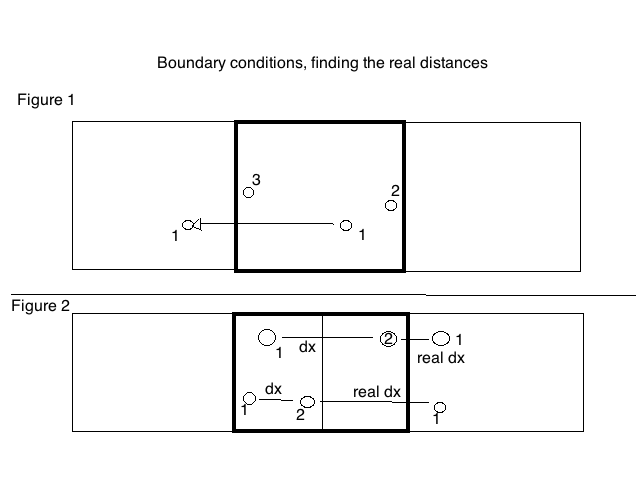
\includegraphics[width = 0.8\textwidth]{/Users/Tuv/Documents/Programming/FYS3150/Project5/molecular-dynamics-fys3150-master/Boundaryconditions.png}
\caption{In figure 1 we see an atom moving through the boundary of our volume. When the atom moves through the boundary we have to move the initial position (1) to be able to calculate the real distance of the atom from the initial position.
In figure 2 we see the real distances of dx when an atom has moved through the boundary. Atom 1 reappears on the other side of the volume, but we want int to be able to "continue" trough the boundary. }
\end{figure}
\subsubsection{Optimization}
Disclamer: Because of limited time, this subsection was not implementet in the code, but is highly recommended for large simulations.\\
\\
Because the lennard-jones potential goes quickly to zero, it is possible to implement a maximum distance $r_{cut}$ where the distance between two atoms is big enough for the potential and hence the force between the atoms to be close to zero. Iterating over atoms who are to far away to exert any force on the atom we are looking at is a waste of computing power.\\
We can implement this by making a list of the closest neighbours to the atom, the ones who are inside the $r_{cut}$ distance, and only iterating over these atoms. It is important to keep in mind that for every timestep, atoms can enter or exit the $r_{cut}$ distance and the neighbour list must be updated.
\newpage
\section{Results}

All the results was simulated with a lattice containing $4\times 7\times 7\times 7 = 1372$ atoms. It ran for 20 000 time-steps with $\Delta t = 10^{-14}$s  and used initial temperatures from 500 K - 1530 K with $\Delta T = 10$\\ 

\begin{figure}[H]
\centering
\subfloat[Initial temperature = 500 K]{\includegraphics[width=0.7\textwidth]{/Users/Tuv/Documents/Programming/FYS3150/Project5/build-molecular-dynamics-fys3150-Desktop_Qt_5_7_0_clang_64bit-Release/EnergyplotInitialTemperature=500.png}}\\
\subfloat[Initial temperature = 700 K]{\includegraphics[width=0.7\textwidth]{/Users/Tuv/Documents/Programming/FYS3150/Project5/build-molecular-dynamics-fys3150-Desktop_Qt_5_7_0_clang_64bit-Release/EnergyplotInitialTemperature=700.png}}
\caption{Plot of kinetic, potential and total energy showing the energy is conserved.}
\end{figure}

\begin{figure}[H]
\centering
\includegraphics[width=0.8\textwidth]{/Users/Tuv/Documents/Programming/FYS3150/Project5/build-molecular-dynamics-fys3150-Desktop_Qt_5_7_0_clang_64bit-Release/TemperatureratiovsTime.png}
\caption{Time-evolution of the temperatureratio $T/T_{initial}$ for different initial temperatures}
\end{figure}



\begin{figure}[H]
\centering
\includegraphics[width=0.8\textwidth]{/Users/Tuv/Documents/Programming/FYS3150/Project5/build-molecular-dynamics-fys3150-Desktop_Qt_5_7_0_clang_64bit-Release/TemperatureratiovsTemperature.png}
\caption{Temperature when the system reaches equilibrium devided by the initial 
temperature of the system $T_{final}/T_{initial}$, ploted agaist the temperature at equilibrium $T_{final}$. We see indication of a phase transition around 300 K}
\end{figure}

\begin{figure}[H]
\centering
\includegraphics[width=0.8\textwidth]{/Users/Tuv/Documents/Programming/FYS3150/Project5/build-molecular-dynamics-fys3150-Desktop_Qt_5_7_0_clang_64bit-Release/RSquaredvsTime.png}
\caption{The squared distance between atoms as a fuction of time. We find the diffusion constant by finding the slope of the curves}
\end{figure}

\begin{figure}[H]
\centering
\includegraphics[width=0.8\textwidth]{/Users/Tuv/Documents/Programming/FYS3150/Project5/build-molecular-dynamics-fys3150-Desktop_Qt_5_7_0_clang_64bit-Release/DiffusionvsTime.png}
\caption{Diffusion constant as a function of time. Higher initial temperatures gives a higher diffusion constant. }
\end{figure}

\begin{figure}[H]
\includegraphics[width=0.8\textwidth]{/Users/Tuv/Documents/Programming/FYS3150/Project5/build-molecular-dynamics-fys3150-Desktop_Qt_5_7_0_clang_64bit-Release/TemperatureDiffusionConstantlast.png}
\caption{The diffusion constant at the final timestep vs the temperature at equilibrium $T_{final}$. We see a clear phase transition around 300 K.}
\end{figure}
\newpage
\section{Discussion}
\subsection{Conservation of Energy}
We wanted to work with the microcanonical ensemble, which means we need to ensure that the number of particles N, the volume V and the energy E is constant. By using periodic boundary conditions we fix the volume based on our value of the lattice constant, the number of particles is also fixed because every particle that exits the volume reappears on the oppsite side of the volume. In figure 5 I have plotted the kinetic, potential and total energy and as we can see the energies are also conserved, which means we have a microcanonical ensemble.
\subsection{Temperaturevariations}

I imagine initializing the argon-crystal by having it in a state with absolutely no energy, then in a infinitely short moment zapping every single atom with a very large amount of energy and just as fast removing the energy source. Every atom now have a large amount of kinetic energy, but they are trapped in the well of the lennard-jones potential. If the energy given to the atoms are big enough for them to climb out of the potential well, we get a phase transition because they can now move freely to greater distances like a gas. If the atoms does not get enough energy they will forever be trapped in the potential well, moving back and forth (See figure 3 of the Lennard-Jones potential). Even though I imagine the movement of an atom climbing up the hill of the potential in figure 3, it is ofcourse just a way of interpreting an atom moving back and forth between other atoms beeing pushed away if it gets too close to another and being pulled back if it gets too far away.\\

In figure 6 we have plotted different initial temperatures as a function of time. We can see that for every initial temperature the temperature falls  very quickly in the beginning, which makes sense because every atom has to fight the potential well and loses kinetic energy in the process, or to be more precise the attractive forces of the atoms in close proximity are trying to hold the atom back.There is however a big difference in how low the temperature gets before stabelizing around half the initial temperature. We can see that for very high initial temperatures the temperature does not fall much under half the initial temperature. We initialize every atom with the Boltzmann speed distribution and for higher initial temperatures there is a bigger probability that an atom has a very high kinetic energy and climbes directly out of the potential and break their bonds with the nearby atoms. Some of the atoms will, however, alwas have velocity in the oposite direction and try climbing towards infinty, that is have a direction towards another atom. Because of the immense repulsive forces the atom will eventually lose all it's kinetic energy and turn around. Because of this, some atoms use a longer time to climb out of potential and the temperature will always fall below the 0.5 mark before stabelizing around 0.5.\\

This plot does not however show us much about any phase-transition in the system. To look closer at this we plot the temperature ratio of $T_{final}/T_{initial}$ vs $T_{final}$ (figure 7). \\
We see now that there is a sudden drop in the plot around 300 K, this indicates a sudden change in the properties of the system. We look closer at this in the next section.
\subsection{The Diffusion Constant}
We calculated the diffusion constant from equation 12 which is just the slope of the $r^2 (t)$ curve as the time goes to infity. We are not able to make the time move to infity, but we will settle for an estimate. In figure 8 we have plotted some selected values of $r^2(t)$ based on the result we found in figure 7. As we can see, for an initial temperature of 590 K, the square distance does not increase, which indicates that the atoms has not recieved enough energy to escape from the potential well and are still trapped close to the initial position. When increasing to 600 K and beyond we see that the atoms finally escapes the well because they now move further away from the initial position. We can also see that the greater the initial temperature, the faster they escape from the well and start moving further away.\\

In figure 9 the diffusion constant is plotted against time for different initial temperatures. We see that the constant stabelizes at higher values for higher temperatures. However, because we are not able to let the time move to infity the values in this plot are very approximate. For instance would the curve for T = 500 K eventually reach zero because the temperature is not high enough for the atoms to escape the potential well.\\

Finally we look at figure 10 where the diffusion constant is plotted against the final temperatures. We can now see that for final temperatures lower than 300 K the diffusion constant is stable close to zero, again they would be zero if we would let the simulation run for a very long time, but we see now very clearly that for final temperature higher than 300 K we get a phase transition and the diffusion constant stabelizes at at higher values.\\

The results correspond nicely with our expectations, but we would benefit from simulating over a greater timeperiod.
\newpage
\section{Conclusion}
The goal of this project was to investigate the properties of an argon liquid and find the temperature where the phase transition occurs.\\
We found the density $\rho$ to be constant at 1823.25 $kg/m^{3}$ and the energy was conserved for different initial temperatures. In other words, N, V and E is conserved and we are looking at the microcanonical ensemble.\\

When looking at the temperaturevariations we found that the ratio of $T_{final}/T_{initial}$ is stable around 0.5 except at 300 K, where it suddenly drops, before climbing back up to 0.5 for higher temperatures. For future calculations it is a good idea to increase the number of timesteps and reduce the steplength. We have very large fluctuations in our plots and even though there is a clear drop in the temperature ratio at 300 K, the uncertainty in the measurements makes it hard to find an exact values of the phase transition. In addition it would be interesting to increasing the  max and min values of $T_{initial}$ to see if there is any drops in the ratio at different temperatures than 300 K. Because we do not simulate over a bigger range of $T$ values we can not say for certain that the drop in the ratio is not just a nummerical error or a coincidence. However, because of the large pressure in the liquid we would expect the phase transition to happen at a higher temperature than the values listed in the internet tables\cite{Argon} and 300 K seems like a reasonable values.\\

The value of the phase transition is again confirmed when looking at the plot of the diffusion constant against final temperatures. But again we have to acknowledge to uncertainty in our simulation because of the short timespan we are using in the simulation. For the the diffusion constant to be exact we need to simulate for an inifinitely long timeinterval. When working with statistical mechanics, our precision will always increase by gathering more data.


\newpage
\begin{thebibliography}{H}
\bibitem{MD}
\url{https://en.wikipedia.org/wiki/Molecular_dynamics}

\bibitem{Equipartition}
Schroeder, Daniel V.
\emph{An introduction to thermal physcs}
San Francisco, California,
200, p.15
\bibitem{ArgonBoiling}
\url{http://www.chemicalelements.com/elements/ar.html}

\bibitem{Argon}
\url{https://en.wikipedia.org/wiki/Van_der_Waals_constants_(data_page)}

\bibitem{PVdiagram}
\url{http://www.nature.com/articles/srep15850/figures/1}

\bibitem{LennardJones}
 B. Smit,
  \emph{Phase diagrams of Lennard-Jones fluids},
  Amsterdam, Netherlands,
  1992, p.1.
  
\bibitem{DiffusionConstant}
Ursell, Tristan S.,
	\emph{The Diffusion Equation, A multi-dimensional Tutorial},
	California Insitute of Technology, Pasadena,
	2007, p.10.
	\url{http://www.rpgroup.caltech.edu/~natsirt/aph162/diffusion_old.pdf}

\end{thebibliography}


\end{document}
